%!TEX root = main.tex

\subsection{Big Stream Processing Systems}
\label{sec:tut_systems}
%\begin{alltt}TODO\scriptsize 0.75/1 pages
%\end{alltt}

This tutorial started by identifying the most differentiating characteristic of scalable data stream processing systems, which is the notion of data as a continuous, possibly infinite resource instead of ``facts and statistics organized and collected together for future reference or analysis''\footnote{Google Dictionary}. In fact, data stream processing systems broaden the context from retrospective data analysis to continuous, unbounded processing coupled with scalable and persistent application state.  Various forms of stream processing have been employed in the past within their respective domains, such as network-centric processing on byte streams, functional (e.g., monads) and actor programming, complex event processing, and database materialized views. Besides, \emph{stream management} has been an active research field for many years~\cite{abadi2003aurora,arasu_babu_widom_2006,chandrasekaran2003telegraphcq}. Nonetheless, several of these ideas have  only just recently been put together in a consistent manner to compose a stack  centered around the notion of data as an unbounded partitioned stream of records (Figure~\ref{fig:streamstack}). Most importantly, stream processing did not restrict but complemented existing scalable processing models (e.g., MapReduce \cite{dean2008mapreduce}) with persistent partitioned state, time domains, and flexible scoping via \mbox{windows}. The general programming stack  addresses storage, compute, and domain-specific library support.

\begin{figure}[t]
\centering
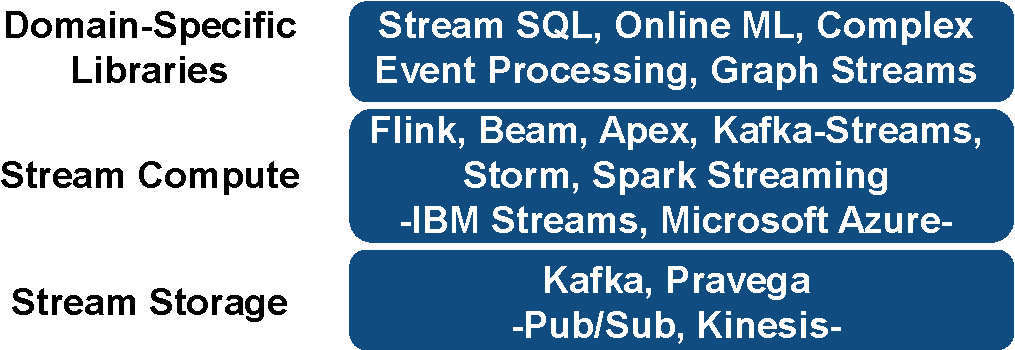
\includegraphics[width=0.4 \textwidth]{pictures/streamstack.pdf}
\vspace*{-2mm}
\caption{The Stack of Scalable Stream Processing}
\label{fig:streamstack}
\vspace*{-5mm}
\end{figure}

\para{Stream Storage.} Data dissemination from consumers to producers is a problem that has been revisited multiple times with different assumptions and needs in mind. In the context of data streaming, direct communication (e.g., TCP channels) was not an option despite low-latency requirements, since it required application ingestion to be actively in sync with data creation while also lacking the transparency and durability of today's cloud computing ecosystem. Furthermore, message brokers (e.g., \name{RabbitMQ}, \name{JMS}) were insufficient for the needs of supporting multiple applications and configurations (i.e., task parallelism). Thus, a class of open-source stream storage systems based on \emph{partitioned replicated logs} was introduced, led by \name{Apache Kafka}~\cite{kreps2011kafka} and more recently \name{Pravega}\footnote{\url{http://pravega.io/}} as well as proprietary cloud services such as \name{Amazon Kinesis}\footnote{\url{https://aws.amazon.com/kinesis/}}. Partitioned replicated logs provide high sequential read and write throughput by exploiting copy-on-write and strict data-parallel access by distinct consumers. Furthermore, they perform offset-based bookkeeping of data access for the purposes of data reprocessing, reconfiguration, and roll-backs, among others. Finally, more effort has been devoted to supporting transactional logging and repartitioning, allowing for seamless integration with modern stream compute systems.

\para{Stream Compute.} We further divide compute into \emph{programming models} and \emph{runtime engines}. In terms of programming model support, there has been a shift from purely event-based, compositional models (e.g., \name{Apache Storm} \cite{toshniwal_et_al_2014}) to more declarative representations~\cite{akidau2015dataflow,carbone_et_al_2015,zaharia_et_al_2013}. Currently, most standard APIs are fluid, functional, and allow declaring relational transformations (e.g., joins, filters) while providing first-class support for persistent partitioned state, stream windows, and event-time prog\-ress using watermarks. The latter allowed application logic to incorporate timers that operate consistently on different time domains (e.g., origin-time), thus allowing out-of-order processing~\cite{li2008out},  a concept popularized, among others, by Google \cite{millwheel,akidau2015dataflow}.

With respect to runtime engines, we observe converging commonalities
such as a dataflow execution model, explicit locally embedded state
(using log-compaction trees \cite{CUSTOM:web/rocksdb}), and
asynchronous snapshots for fault tolerance and
reconfiguration~\cite{state2017carbone,jacques2016consistent}. \name{Spark
  Streaming} \cite{zaharia_et_al_2013}, as a special case, emulates
streaming by slicing computation into recurring batch jobs, yet, it
currently makes use of locally embedded state and there are plans to
adopt a continuous processing runtime for low-latency data streaming.

\iffalse
\para{Domain-Specific Libraries.} A concluding discussion in this tutorial addressed the prospects of standardizing domain-specific libraries such as Stream SQL, CEP, Online Machine Learning and User-Defined Windows \cite{carbone2015cutty} as well as system runtime concepts that are indirectly exposed to the user such as state snapshots \cite{state2017carbone}. Several of these initiatives can already be observed in the effort of Apache Beam \cite{CUSTOM:web/beam} and Calcite \cite{CUSTOM:web/calcite} to serve as standard cross-engine frameworks supported by different runtimes \cite{CUSTOM:web/beamcapabilitymatrix}.
\fi 
